\documentclass[10pt,twocolumn,letterpaper]{article}

\usepackage{cvpr}              % CVPR 官方样式 (cvpr-org/author-kit)
\usepackage{graphicx}
\usepackage{amsmath}
\usepackage{amssymb}
\usepackage{booktabs}
\usepackage{xcolor}
\usepackage{array}

% ---- 中文支持：xeCJK + Noto CJK (需用 xelatex 编译) ----
\usepackage{xeCJK}
\setCJKmainfont{Noto Serif CJK SC}
\setCJKsansfont{Noto Sans CJK SC}
% 无 CJK 等宽字体可用；本文 \texttt{} 内均为 ASCII，故回落到 CJK 无衬线
\setCJKmonofont{Noto Sans CJK SC}
\XeTeXlinebreaklocale "zh"
\XeTeXlinebreakskip = 0pt plus 1pt

\definecolor{cvprlink}{rgb}{0,0.3,0.7}
\usepackage[pagebackref,breaklinks,colorlinks,
            citecolor=cvprlink,linkcolor=cvprlink,urlcolor=cvprlink]{hyperref}

\def\paperID{1}
\def\confName{CVPR}
\def\confYear{2026}

\begin{document}

\title{作业一：文本分类实现\\
\large 词袋模型、Word2Vec 与 BERT 在 NYT 新闻分类上的比较}

\author{自然语言处理课程作业\\
{\tt\small NYT 新闻主题分类}
}

\maketitle

\begin{abstract}
本文在 New York Times (NYT) 新闻数据集上实现并比较了三类文本表示方法：
Bag-of-Words（任务一）、100 维词向量平均（任务二）、
以及微调 \texttt{bert-base-uncased}（任务三）。
NYT 数据按 80\%/10\%/10\% 随机划分为训练、验证与测试集，
全部七组实验共享同一份划分，最终性能统一在测试集上用 Accuracy 与 Macro-F1 评价。

结果显示：预训练 GloVe 词向量平均取得最高的 Macro-F1（0.9770），
Binary BoW 与 Word Frequency 紧随其后（0.9738 / 0.9737），
微调 BERT 最低（0.9433）。
我们分析了 BERT 表现不及预期的原因：
作业指定的 \texttt{max\_length}=64 使 BERT 只能读到每篇文档中位 7.6\% 的内容，
而其余方法均使用全文；
在同等 64-token 预算下 BERT 反而优于其余方法。
\end{abstract}

% ------------------------------------------------------------------ %
\section{实验设置}
\label{sec:setup}

\subsection{数据集}

\textbf{NYT}（\texttt{nyt.csv}）含 11{,}519 篇新闻，两列 \texttt{text} 与 \texttt{label}，
共 3 个类别。数据分布与文档长度如下，这两点对后文分析都很关键：

\begin{center}\small
\begin{tabular}{lrr}
\toprule
类别 & 样本数 & 占比 \\
\midrule
sports   & 8{,}639 & 75.0\% \\
politics & 1{,}451 & 12.6\% \\
business & 1{,}429 & 12.4\% \\
\midrule
\multicolumn{3}{l}{文档长度：均值 638 词，中位 672，p95 1{,}011} \\
\bottomrule
\end{tabular}
\end{center}

类别分布不均衡（最多/最少 $=6.0$），且文档较长（中位 672 词）。

\textbf{AG News}（\texttt{ag.csv}）含 90{,}000 条新闻文本
（均值 39 词，共 4.05M token），按作业要求仅用于训练 Word2Vec 词向量。

\subsection{数据划分}

按作业要求，先对 NYT 数据整体随机打乱（固定随机种子 42），再按 80/10/10 划分：

\begin{center}\small
\begin{tabular}{lrrrr}
\toprule
划分 & 规模 & business & politics & sports \\
\midrule
训练集 (80\%) & 9{,}215 & 1{,}157 & 1{,}134 & 6{,}924 \\
验证集 (10\%) & 1{,}151 & 124 & 152 & 875 \\
测试集 (10\%) & 1{,}153 & 148 & 165 & 840 \\
\bottomrule
\end{tabular}
\end{center}

全部实验通过同一个函数（\texttt{common.get\_splits}）导入该划分，
以保证不同方法之间具有可比性；最终性能统一在测试集上评价。
随机打乱后各划分的类别比例与整体基本一致。

\subsection{评价指标}

\textbf{Accuracy} 为分类正确的样本数占全部测试样本数的比例。
\textbf{Macro-F1} 分别计算每个类别的 F1 后取算术平均。
在本数据上二者的区分能力差距明显：
一个恒预测多数类 \emph{sports} 的退化分类器 Accuracy 已达 0.7285，
但 Macro-F1 仅 0.2810。
因此对本任务而言 Macro-F1 更能反映模型在各类别上的真实能力~\cite{he2008learning}，
后文分析以 Macro-F1 为主。

\subsection{分词}

按作业提示，统一使用 \texttt{nltk.word\_tokenize}~\cite{bird2009nltk}
对小写化文本分词。任务一与任务二共享同一份缓存的分词结果，
使两者的词表来自完全相同的 token。
未做停用词过滤与词干化：作业未要求，
且省略后三种词袋变体仅在加权方式上不同，便于归因。

% ------------------------------------------------------------------ %
\section{任务一：Bag of Words}
\label{sec:task1}

\subsection{方法}

词表在训练语料上构建，大小 $|V| = 127{,}767$；
每篇文档表示为一个 $|V|$ 维向量（稀疏度 0.25\%）。
三种加权方式下，文档 $d$ 向量的第 $i$ 维为：
\begin{align}
\text{Binary BoW:}\quad & x_i = \mathbb{1}[w_i \in d] \\
\text{Word Frequency:}\quad & x_i = c_i = \mathrm{count}(w_i, d) \\
\text{TF-IDF:}\quad & x_i = \mathrm{tf}(w_i,d)\cdot \log\frac{N}{\mathrm{df}(w_i)}
\end{align}
即 Binary BoW 只考虑单词是否出现，Word Frequency 记录出现次数。
分类器统一为 Logistic Regression~\cite{pedregosa2011scikit}
（\texttt{max\_iter}=1000，其余为默认设置）。

词表只在\emph{训练集}上构建，再原样应用到验证集与测试集；
若在全部数据上构建词表会把测试集信息引入特征空间。

\textbf{关于第三种方法。}作业要求三种 Bag-of-Words 方法，
正文明确给出了 Binary Bag of Words 与 Word Frequency 两种，
第三种我们取该族的标准变体 TF-IDF~\cite{salton1988term}。

\subsection{结果}

\begin{center}\small
\begin{tabular}{lcc}
\toprule
表示方法 & Accuracy & Macro-F1 \\
\midrule
Binary Bag of Words & \textbf{0.9887} & \textbf{0.9738} \\
Word Frequency      & 0.9879 & 0.9737 \\
TF-IDF              & 0.9809 & 0.9613 \\
\bottomrule
\end{tabular}
\end{center}

\subsection{分析}

Binary 与 Word Frequency 几乎完全相同（Macro-F1 0.9738 vs 0.9737，
相差约一篇文档）。这对长文档的主题分类是符合预期的：
判断一篇文档是否属于 \emph{sports}，
关键在于 \emph{goal}、\emph{striker} 这类词是否\emph{出现}，
而不在于它们出现了多少次；
词频在首次出现之后提供的额外信息很少，所以二值化几乎不损失可用信息。

TF-IDF 是三者中最低的，这一点初看反直觉。
按类别拆开看（图~\ref{fig:perclass}）可以定位到损失来源：
\emph{business} 的 F1 从 0.9586 降到 0.9324，而 \emph{sports} 几乎不变。
IDF 会降低在许多文档中都出现的词的权重；
由于 \emph{sports} 占训练集的 75\%，
business 与 politics 的普通词汇相对更"稀有"因而被\emph{提高}权重，
而真正能稳定区分这两个少数类的中频词却被压低。
在类别均衡的语料上 TF-IDF 通常是有益的，
但在 6:1 不平衡下它的文档频率先验对少数类不利。

% ------------------------------------------------------------------ %
\begin{figure*}[t]
\centering
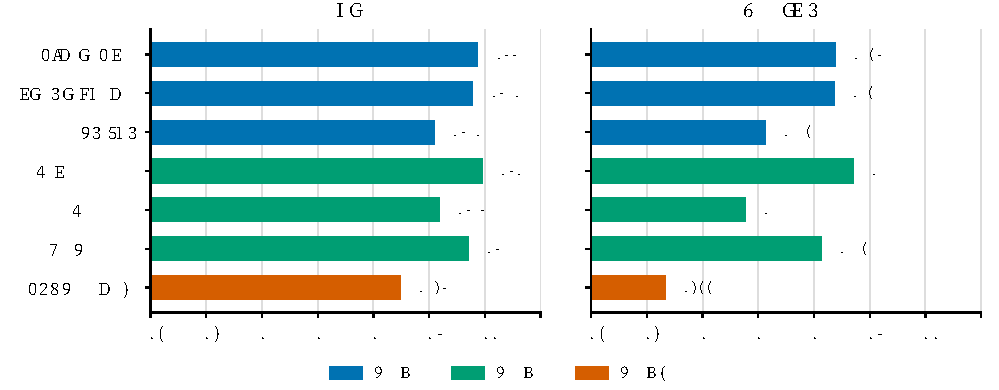
\includegraphics[width=\textwidth]{fig/main_comparison.pdf}
\caption{NYT 测试集上七组实验的 Accuracy 与 Macro-F1。
注意横轴从 0.93 起截断。Accuracy 把七种方法压缩在 0.975--0.990，
而 Macro-F1 拉开到 0.943--0.977。}
\label{fig:main}
\end{figure*}

\section{任务二：Word2Vec}
\label{sec:task2}

\subsection{方法}

对一篇含 $n$ 个有效单词（即在词向量词表内的词）的文档，
其词向量为 $e(w_1), \dots, e(w_n)$，文档向量取平均：
\begin{equation}
e(d) = \frac{1}{n}\sum_{i=1}^{n} e(w_i)
\end{equation}
词向量维度统一为 100，分类器仍为 Logistic Regression。
三种词向量来源：

\begin{enumerate}\itemsep2pt
\item \textbf{预训练 GloVe}：\texttt{glove.6B.100d}~\cite{pennington2014glove}，
词表 400{,}001。
\item \textbf{AG News 训练的 Word2Vec}：用 gensim~\cite{rehurek2010gensim}
在 90{,}000 条 AG News 文本上训练，
skip-gram~\cite{mikolov2013word2vec,mikolov2013efficient}，
\texttt{vector\_size}=100，\texttt{window}=5，\texttt{min\_count}=2，10 轮。
\item \textbf{NYT 训练的 Word2Vec}：同样的超参，在 NYT 文本上训练。
\end{enumerate}

平均时跳过不在词向量词表内的词；若一篇文档全部词都不在词表内则回落为零向量
（本实验中未发生）。因平均后的稠密特征未经缩放会显著减慢 lbfgs 收敛，
在 Logistic Regression 前加一步标准化。

\textbf{避免信息泄漏。}第 3 组的 NYT Word2Vec 只在\emph{训练集}文本上训练。
若用全部 11{,}519 篇训练，测试集的词共现统计会影响词向量本身，
使测试结果偏乐观。

\textbf{可复现性。}Word2Vec 使用 \texttt{workers}=1。
多线程下 gensim 的参数更新顺序不确定，
即使固定随机种子，重复运行的 Macro-F1 仍会波动最多 0.007——
与本文讨论的部分差异同量级。
单线程训练代价为几分钟，换来结果的精确可复现（已由两次独立运行验证）。

\subsection{结果}

\begin{center}\small
\begin{tabular}{lrcc}
\toprule
词向量来源 & 覆盖率 & Accuracy & Macro-F1 \\
\midrule
预训练 GloVe        & 98.1\% & \textbf{0.9896} & \textbf{0.9770} \\
Word2Vec on NYT     & 98.4\% & 0.9870 & 0.9713 \\
Word2Vec on AG News & 95.5\% & 0.9818 & 0.9577 \\
\bottomrule
\end{tabular}
\end{center}

覆盖率为测试集中能在词向量词表内找到的 token 比例。

\subsection{分析}

预训练 GloVe 是全部七组实验中 Macro-F1 最高的，
尽管它完全是通用词向量、从未见过 NYT 语料。
其优势来自预训练规模：6B token 的语料与 400k 词表，
使那些区分 business 与 politics 的中频词也能得到良好估计，
而 Macro-F1 的差距恰恰产生在这些词上。

两个自训练模型的对比则分离出另一个因素：

\begin{itemize}\itemsep2pt
\item \textbf{领域匹配比语料规模更重要。}
NYT 训练的词向量（6.7M token）明显优于 AG News 训练的（4.1M token），
0.9713 vs 0.9577。算法、维度、token 量级都接近，
差别在于一个是在目标领域上训练的——它 98.4\% 的覆盖率也是三者中最高的。
\item \textbf{但规模仍胜过领域匹配。}
NYT 自训练词向量仍不及通用 GloVe。
6.7M token 的语料对于估计 57k 个词的 100 维向量来说偏小，
无论领域多么匹配。
\end{itemize}

AG News 迁移效果最差还有一个结构性原因：
其文本平均仅 39 词（标题加首句），
共现统计来自短标题式的上下文，
而 NYT 是约 670 词的长篇报道——词表与语域双重不匹配。

与任务一对比：100 维的词向量平均达到了与 127{,}767 维稀疏词袋相当甚至更好的效果
（GloVe 0.9770 vs Binary BoW 0.9738），
维度相差约 1278 倍。这体现了稠密分布式表示在维度效率上的优势。
但也应注意词向量并未\emph{大幅}超过词袋模型——
在只有 3 类、文档较长的主题分类任务上，词汇重叠本身已提供了几乎足够的信号。

% ------------------------------------------------------------------ %
\section{任务三：BERT 微调}
\label{sec:task3}

\subsection{方法}

按作业要求使用 \texttt{google-bert/bert-base-uncased}~\cite{devlin2019bert}，
\texttt{max\_length}=64，训练 3 epochs。
其余设置遵循标准 BERT 微调配方~\cite{sun2019finetune}：
batch size 32，AdamW~\cite{loshchilov2019decoupled} 学习率 $2\times10^{-5}$，
weight decay 0.01（bias 与 LayerNorm 除外），
10\% 线性 warmup，梯度裁剪 1.0，fp16。
使用显式的 PyTorch 训练循环而非 \texttt{Trainer}，使流程完全可见，
且不依赖在不同 transformers 版本间有变动的 Trainer API。
单张 H20 GPU 上 288 steps/epoch、共 864 steps，训练约 35 秒。

\subsection{结果}

\begin{center}\small
\begin{tabular}{crrr}
\toprule
Epoch & 训练损失 & 验证 Accuracy & 验证 Macro-F1 \\
\midrule
1 & 0.2816 & 0.9765 & 0.9422 \\
2 & 0.0462 & 0.9757 & 0.9433 \\
3 & 0.0175 & 0.9757 & 0.9424 \\
\midrule
\multicolumn{2}{l}{\textbf{测试集（3 epochs 后）}}
  & \textbf{0.9748} & \textbf{0.9433} \\
\bottomrule
\end{tabular}
\end{center}

\begin{figure}[t]
\centering
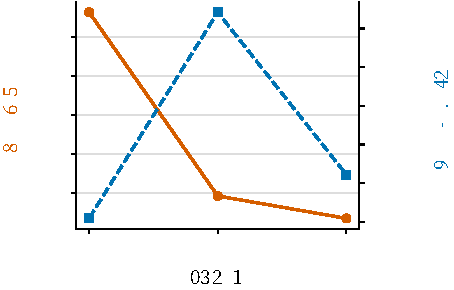
\includegraphics[width=\linewidth]{fig/bert_training.pdf}
\caption{BERT 微调过程。训练损失下降约 16 倍，
而验证 Macro-F1 始终持平在 0.942 左右。}
\label{fig:bertcurve}
\end{figure}

如图~\ref{fig:bertcurve}，3 轮中训练损失从 0.2816 降到 0.0175（约 16 倍），
但验证 Macro-F1 始终在 0.942 附近没有改善。
模型在训练数据上拟合得越来越好却没有更好地泛化，
这是输入信息已被利用完毕的特征，而非训练不足。

% ------------------------------------------------------------------ %
\section{比较与分析}
\label{sec:analysis}

\subsection{总体比较}

\begin{table}[t]
\centering\small
\caption{NYT 测试集上七组实验的最终结果，按 Macro-F1 降序。}
\label{tab:main}
\begin{tabular}{llcc}
\toprule
任务 & 表示方法 & Accuracy & Macro-F1 \\
\midrule
任务二 & 预训练 GloVe (100d)  & \textbf{0.9896} & \textbf{0.9770} \\
任务一 & Binary Bag of Words  & 0.9887 & 0.9738 \\
任务一 & Word Frequency       & 0.9879 & 0.9737 \\
任务二 & Word2Vec on NYT      & 0.9870 & 0.9713 \\
任务一 & TF-IDF               & 0.9809 & 0.9613 \\
任务二 & Word2Vec on AG News  & 0.9818 & 0.9577 \\
任务三 & BERT-base-uncased    & 0.9748 & 0.9433 \\
\midrule
\multicolumn{2}{l}{\emph{多数类基线（参考）}} & 0.7285 & 0.2810 \\
\bottomrule
\end{tabular}
\end{table}

\begin{figure*}[t]
\centering
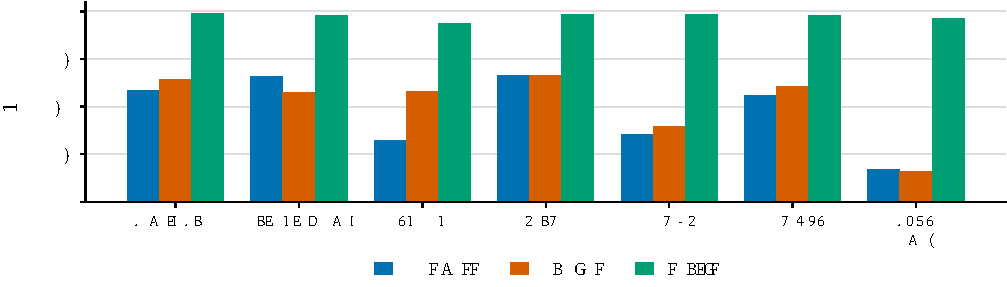
\includegraphics[width=\textwidth]{fig/per_class_f1.pdf}
\caption{各类别 F1。所有方法在多数类 \emph{sports} 上都接近完美（$\ge 0.9935$），
Macro-F1 的全部差异来自 \emph{business} 与 \emph{politics} 两个少数类。}
\label{fig:perclass}
\end{figure*}

\subsection{各类别表现}

如图~\ref{fig:perclass}，所有方法在 \emph{sports} 上的 F1 均 $\ge 0.9935$，
因此 Macro-F1 的全部差异都来自两个少数类。
business 与 politics 的混淆在语义上是真实的
（贸易政策、监管、税收同时属于两个主题），
并且这两类的训练样本最少（各约 1{,}150 篇，对比 \emph{sports} 的 6{,}924 篇）。
这也说明为什么 Macro-F1 在本任务上更有意义：
Accuracy 把七种方法压缩在 0.975--0.990 的窄区间内，
而 Macro-F1 拉开到 0.943--0.977。

\subsection{BERT 为何表现最低}

表~\ref{tab:main} 字面上说：
一个 110M 参数的预训练 Transformer 输给了 100 维词向量取平均。
但这个比较并不公平，而且不公平的程度可以量化。
用 BERT 自己的 WordPiece 分词器~\cite{sennrich2016bpe}
统计测试集全部文档的真实长度：

\begin{center}\small
\begin{tabular}{lr}
\toprule
全文长度中位数（word piece） & 847 \\
全文长度均值 & 819 \\
超过 64 token 的文档 & 1{,}153 / 1{,}153 (100\%) \\
\textbf{BERT 实际读到的比例（中位）} & \textbf{7.6\%} \\
BERT 实际读到的比例（均值） & 10.8\% \\
\bottomrule
\end{tabular}
\end{center}

测试集中\emph{没有一篇文档未被截断}，
BERT 读到的中位比例只有 7.6\%，大致相当于开头一到两句话；
而词袋模型与词向量方法读的是全部约 847 个 token。
所以表~\ref{tab:main} 比较的并不是"模型对模型"，而是"64 token 对全文"。

\begin{figure}[t]
\centering
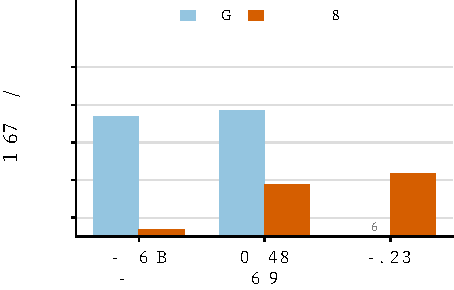
\includegraphics[width=\linewidth]{fig/truncation_control.pdf}
\caption{同等输入预算下的对照实验。
把 Binary BoW 与 GloVe 平均也截断到每篇文档的前 64 个词 token 后，
BERT 由最低变为最高。
BERT 无"全文"对照，因 64 为作业指定设置。}
\label{fig:trunc}
\end{figure}

为验证这一解释，我们把 Binary BoW 与 GloVe 平均也限制为只使用每篇文档的
前 64 个词 token，其余设置不变（图~\ref{fig:trunc}）：

\begin{center}\small
\begin{tabular}{lccr}
\toprule
方法 & 全文 & 前 64 token & $\Delta$ \\
\midrule
Binary BoW & 0.9738 & 0.9138 & $-0.0600$ \\
GloVe 平均 & 0.9770 & 0.9377 & $-0.0393$ \\
BERT       & ---    & \textbf{0.9433} & --- \\
\bottomrule
\end{tabular}
\end{center}

排序发生反转：在同等 64-token 预算下，
BERT（0.9433）高于 GloVe（0.9377）与 Binary BoW（0.9138）。
也就是说，按"单位输入 token 的信息利用效率"衡量，
BERT 是三者中最强的；
它在表~\ref{tab:main} 中排在最后，
是因为指定的 \texttt{max\_length}=64 只给了它约 7.6\% 的证据。
截断使 Binary BoW 损失 0.060、GloVe 损失 0.039 的 Macro-F1，
这直接说明被截去的那 92\% 内容确实携带着所有方法都能利用的判别信号。
这也解释了第~\ref{sec:task3} 节中验证曲线持平的现象：
BERT 并非训练不足，而是已把 64 个可见 token 中的信息利用完毕。

若要在本数据上充分发挥 BERT 的能力，
自然的做法是增大 \texttt{max\_length}（代价是显存与时间随长度增长），
或改用可处理长输入的模型~\cite{beltagy2020longformer}。
本作业指定了 \texttt{max\_length}=64，故未在此展开。

\subsection{运行代价}

\begin{center}\small
\begin{tabular}{llr}
\toprule
方法 & 硬件 & 耗时 \\
\midrule
词袋模型（三种）        & CPU & ${\sim}25$ 秒 \\
GloVe 平均              & CPU & ${\sim}35$ 秒 \\
Word2Vec 训练 (AG/NYT)  & CPU（单线程） & ${\sim}2.5$ / ${\sim}3.7$ 分 \\
BERT 微调（3 epochs）   & 1$\times$ H20 GPU & ${\sim}35$ 秒 \\
\bottomrule
\end{tabular}
\end{center}

GloVe 的耗时主要是加载 347 MB 词向量文件。

% ------------------------------------------------------------------ %
\section{结论}
\label{sec:conclusion}

\begin{enumerate}\itemsep3pt
\item \textbf{Binary BoW 与 Word Frequency 表现几乎相同}（0.9738 / 0.9737）。
对长文档主题分类，词的\emph{出现}承载了主要信号，词频提供的额外信息很少。

\item \textbf{TF-IDF 反而低于原始词频}（0.9613）。
IDF 的文档频率先验与 6:1 的类别不平衡产生了不利的相互作用，
具体损害体现在 \emph{business} 类的 F1 上。

\item \textbf{预训练 GloVe 是效果最好的表示}（Macro-F1 0.9770）。
预训练语料的规模效应胜过领域针对性，
且只需 100 维即可达到甚至超过 127{,}767 维词袋的效果。

\item \textbf{自训练词向量之间，领域匹配比语料规模更重要}：
NYT 训练（0.9713）明显优于 AG News 训练（0.9577）。
AG News 的短文本语域与 NYT 长文差异也是迁移效果差的原因之一。

\item \textbf{BERT 排在最后源于 \texttt{max\_length}=64 的限制，而非模型能力}。
它只能读到每篇文档中位 7.6\% 的内容；
在同等 64-token 预算下它反而优于其余方法（0.9433 vs 0.9377 / 0.9138）。

\item \textbf{Macro-F1 比 Accuracy 更适合评价本任务}。
多数类基线的 Accuracy 已达 0.7285 而 Macro-F1 仅 0.2810；
七种方法的 Accuracy 挤在 0.975--0.990，Macro-F1 则拉开到 0.943--0.977，
差异全部来自两个少数类。
\end{enumerate}

\paragraph{关于数值的说明。}
七种方法的 Macro-F1 均高于 0.94，任务已接近饱和。
1{,}153 篇的测试集对 Macro-F1 的分辨率约为 $\pm 0.01$，
因此 Binary BoW 与 Word Frequency 之间 0.0001 的差距属于噪声，不应作结论；
而 BERT 与 GloVe 之间 0.034 的差距、
以及截断带来的 0.039--0.060 的差距，则远超这一噪声水平。
另需说明，原始数据含 72 篇内容重复的文档，
其中 8 篇在指定的随机划分下横跨训练集与测试集；
为不偏离作业规定的划分流程，我们保留原样。

\paragraph{代码与复现。}
代码运行说明见 \texttt{README.md}。
简要地说，\texttt{bash scripts/setup.sh} 准备环境，
\texttt{bash scripts/download\_assets.sh} 下载 GloVe 与 BERT 权重，
\texttt{bash scripts/run\_all.sh} 依次运行三个任务、生成图表与本 PDF。
各任务的完整指标（含每类 F1 与 \texttt{classification\_report}）
输出在 \texttt{results/*.json}。

{\small
\bibliographystyle{ieeenat_fullname}
\bibliography{refs}
}

\end{document}
